\StartPlate{V06}{Do not truncate the full character}{Deep values, the full compact domain, and a noncompact generator are distinct certificates.}
\begin{center}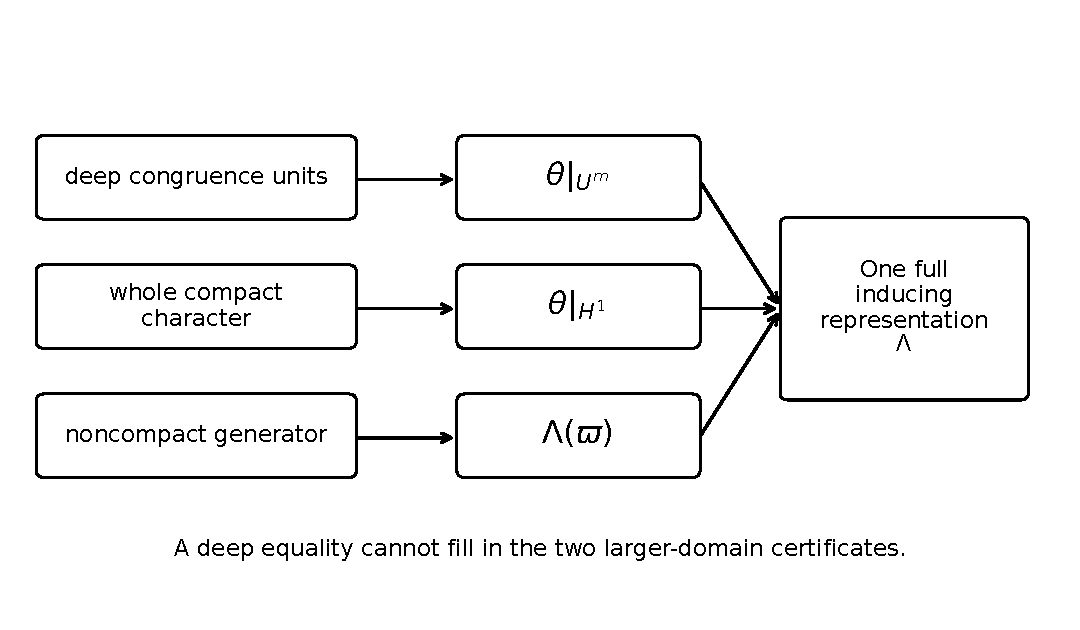
\includegraphics[width=\linewidth]{figures/V06.pdf}\end{center}
A trace expression first describes a character on sufficiently deep congruence units. The full simple character also has values on the larger native unit domain. A full inducing representation retains further central and noncompact data. These are successive obligations, not three interchangeable notations for the same calculation.

The direct character construction transfers the whole preceding character, applies the actual permitted correction, and then checks the intersection needed for shallow extension. The continuation113 correction exhibits why noncompact normalization matters. In exponents of ninth roots of unity,
\[
\nu(\varpi)=\zeta_9,\qquad
\nu(\varpi_F/\varpi^3)=\zeta_3^2
\quad\Longrightarrow\quad \nu(\varpi_F)=1.
\]
Setting $\nu(\varpi)=1$ instead gives $\zeta_3^2$, changing the central character. The accompanying finite check verifies this root-of-unity identity only. The full unit character, intertwining, and type-extension statements retain the arithmetic hypotheses developed in the progress paper.
\vfill\PlateSource{Domain diagram}{Part I, Sections 7.5--8.5; Part II, Section 18}{15}
